% -*- mode:flyspell; mode:latex -*-
\documentclass[12pt]{article}

% \addtolength{\oddsidemargin} {-0.885in}
% \addtolength{\textwidth}{1.75in}
% \addtolength{\evensidemargin}{-0.8in}
% topmargin -0.5in
\usepackage[a4paper, top=1cm, left=1.5cm, right=1.5cm]{geometry} % width= , 

\usepackage[latin1]{inputenc}
\usepackage[T1]{fontenc}
\usepackage[english]{babel}
\usepackage{graphicx}
\usepackage{float}


\usepackage{tikz}
\usepackage{[caption}
\usetikzlibrary{arrows}
\usetikzlibrary{decorations.markings}
\usetikzlibrary{decorations.pathmorphing}
% \usepackage[absolute,overlay]{textpos}
% \usepackage{onimage}

\usepackage{times}
\usepackage{graphics}

% \usepackage{subfigure}
% \usepackage{scalefnt}
%
% \renewcommand\thesubfigure{\arabic{subfigure}}

\usepackage{amsmath}
\usepackage{hyperref}
\usepackage{hhline}
\usepackage{subfig}
\usepackage{color}
\usepackage[all]{hypcap}

\usepackage[normalem]{ulem}  % for striking out
% \usepackage{fancyhdr}
% \pagestyle{fancy}
% \fancyhead[C]{}
% \fancyhead[L] {\it{Mu2e-doc-29670-v1.0} }
%%%%%%%%%%%%%%%%%%%%%%%%%%%%%%%%%%%%%%%%%%%%%%%%%%%%%%%%%%%%%%%%%%%%%%%%%%%%%%
% use natbib - biblatex not available on Mu2e interactive nodes
%%%%%%%%%%%%%%%%%%%%%%%%%%%%%%%%%%%%%%%%%%%%%%%%%%%%%%%%%%%%%%%%%%%%%%%%%%%%%%
\usepackage[square,sort,comma,numbers]{natbib}

% location of the .bib files: env var BIBINPUTS (~/library/bibliography)

% \usepackage[backend=biber, style=numeric-comp, sorting=ynt] {biblatex}
% \addbibresource{clfv.bib}

% \addbibresource{stntuple.bib}
% \addbibresource{mu2e_web.bib}
% \addbibresource{radiative_pion_capture.bib}

\graphicspath{{figures/}}
%%%%%%%%%%%%%%%%%%%%%%%%%%%%%%%%%%%%%%%%%%%%%%%%%%%%%%%%%%%%%%%%%%%%%%%%%%%%%%
% for portability, make sure all commands are included locally
% order them alphabetically
%%%%%%%%%%%%%%%%%%%%%%%%%%%%%%%%%%%%%%%%%%%%%%%%%%%%%%%%%%%%%%%%%%%%%%%%%%%%%%
% \include{commands}

\newcommand {\keVc}       {\mbox{$\rm keV\!/\!c$}}
\newcommand {\kmax}       {\mbox{$k_{\rm max}$}}

\newcommand {\MeVc}       {\mbox{$\rm MeV\!/c$}}
\newcommand {\MeVcsq}     {\mbox{$\rm MeV\!/c^2$}}

\newcommand {\mumemconv}[1][A] {\mbox{$\mu^- \textrm{#1} \rightarrow e^- \textrm{#1}$}}
% Define a relay to have 2 default arguments instead of limit of 1
\newcommand {\mumepconv}[1][A] {%
  \def\ArgI{{#1}}%store the first argument
  \mumepconvRelay
}
\newcommand \mumepconvRelay[1][A]  {\mbox{$\mu^- \textrm{\ArgI} \rightarrow e^+ \textrm{#1}$}}
\newcommand {\muminus}    {\mbox{$\mu^-$}}
\newcommand {\muplus}    {\mbox{$\mu^+$}}
\newcommand {\MuToEm}     {\mbox{$\mu^- \ra e^-$}}
\newcommand {\MuToEp}     {\mbox{$\mu^- \ra e^+$}}
\newcommand {\MuPToEp}    {\mbox{$\mu^+ \ra e^+$}}
\newcommand {\ra}        {\rightarrow}
\newcommand {\tandip}    {\mbox{$\tan \lambda$}}

\newcommand {\Pb}[1]     {\mbox{$\rm ^{#1}Pb$}}                 % isotopes of lead
\newcommand {\Au}[1]     {\mbox{$\rm ^{#1}Au$}}                 % isotopes of gold
\newcommand {\Ir}[1]     {\mbox{$\rm ^{#1}Ir$}}                 % isotopes of iridium
%%%%%%%%%%%%%%%%%%%%%%%%%%%%%%%%%%%%%%%%%%%%%%%%%%%%%%%%%%%%%%%%%%%%%%%%%%%%%%
% editing commands
%%%%%%%%%%%%%%%%%%%%%%%%%%%%%%%%%%%%%%%%%%%%%%%%%%%%%%%%%%%%%%%%%%%%%%%%%%%%%%
\newcommand {\add}[1]    {{\red #1}}
\newcommand {\alt}[1]    {{\green #1}} %alternate comment color
\newcommand {\del}[1]    {{\blue \sout{#1}}}
\newcommand {\dlt}[1]    {{\violet \sout{#1}}} %alternate delete color

\newcommand {\black}     {\color{black}}
\newcommand {\red}       {\color{red}}
\newcommand {\blue}      {\color{blue}}
\newcommand {\strike}[1] {{\blue \sout{#1}}}
%%%%%%%%%%%%%%%%%%%%%%%%%%%%%%%%%%%%%%%%%%%%%%%%%%%%%%%%%%%%%%%%%%%%%%%%%%%%%%
\begin{document}

\begin{titlepage}
  \begin{flushright}
    \bf {MU2E/PHYSICS/40523} \\
    version 1.01
    \today
 \end{flushright}

  \vspace{1cm}

  \begin{center}
    {\Large \bf Mu2e 2020 sensitivity update.

      \vspace{0.3in}

      11. Beam-related backgrounds
    }

    \vspace{1cm}

    P. Murat(FNAL)

    % \footnote{\texttt{Fermilab; e-mail: murat@fnal.gov}}
    \vspace{0.3cm}

    \vspace{0.8cm}
  \end{center}

  \begin{abstract}
    This note presents an estimate of the beam-associated background in \MuToEm\ channel
    for the Mu2e 2020 sensitivity update (SU2020).
    \vspace{0.2in}
  \end{abstract}

\end{titlepage}
% \frontmatter
% \chapter*{Abstract}
%
% \addcontentsline{toc}{chapter}{Abstract}
%
% \mainmatter
%
{\tableofcontents}

%%%%%%%%%%%%%%%%%%%%%%%%%%%%%%%%%%%%%%%%%%%%%%%%%%%%%%%%%%%%%%%%%%%%%%%%%%%%%%%
%\chapter{Calibration}
%%%%%%%%%%%%%%%%%%%%%%%%%%%%%%%%%%%%%%%%%%%%%%%%%%%%%%%%%%%%%%%%%%%%%%%%%%%%%%%
% \input{input_data}

%%%%%%%%%%%%%%%%%%%%%%%%%%%%%%%%%%%%%%%%%%%%%%%%%%%%%%%%%%%%%%%%%%%%%%%%%%%%%%%
\newpage
\section {Revision history}
\begin{itemize}
\item
  v1.01: initial version
\end{itemize}

%%%%%%%%%%%%%%%%%%%%%%%%%%%%%%%%%%%%%%%%%%%%%%%%%%%%%%%%%%%%%%%%%%%%%%%%%%%%%%
\section {Introduction}

In this note, we outline a data-driven approach to understanding the vertical alignment of the
Mu2e beamline.

The efficiency of particle transport through the Mu2e beamline depends on the beamline
alignment. As particles moving through the transport solenoid drift vertically,
the transport efficiency more sensitive to the vertical alignment more important than
to horizontal one.

For different particle species, the sensitivity of the transport efficiency to misalignment
is different. Probably, the most sensitive to the vertical alignment is the antiproton
transport efficiency and the expected antiproton background.
% 
The most important parameters defining the antiproton transport efficiency are relative
vertical positions of the production target, the TS1 collimator, the TS3 collimator,
and the stopping target. For example, a vertical displacement of the TS3 collimator 
with respect to the production target by a few centimeters could increase the antiproton
background by an order of magnitude. A change of the PS magnetic field resulting 
in a similar vertical displacement of the transported particles would have the same impact.

It is therefore quite important to develop data-driven techniques to understand and control
the vertical alignment of the beamline.

%%%%%%%%%%%%%%%%%%%%%%%%%%%%%%%%%%%%%%%%%%%%%%%%%%%%%%%%%%%%%%%%%%%%%%%%%%%%%% 
\section {Simulation strategy}

Trace events till the VD9. At that point, select events with P>100 MeV/c electrons.
Resample by a needed factor.
Keep in mind that the probability to scatter and make hits in the tracker is $< 1 \times 10^{-5}$.
Therefore, starting from VD9, need to run at least $10^6$ events.

As the goal is to produce an upper bound, try not to run reconstruction, just the simulation.
It might work.

Simulation stages:

\begin{itemize}
\item
  Stage1 : proton interactions in the production target --> before TS31 collimator 
\item
  Stage2 : before TS31 collimator -> before TS5 collimator
\item
  Stage3 : before TS5 collimator --> VD9
\item
  Stage4 : before VD9 --> tracker mother volume
\item
  Stage5 : hit simulation, digitization. Count events with 20+ hits produced by a 100 MeV/c+ electron
\end{itemize}

\begin{itemize}
\item [stage 1]
  generate $1 \times 10^9$ POT, output of stage 1: bmum0s11b0
\item
  to reduce computing effort,
  after stage 1, strip events with muons P > 70 MeV/c : bmum0s1b. 
  Only these may produce 100 MeV/c electrons
\item
  after stage 1, strip events with electrons P > 100 MeV/c : bmum0s16b0. Trace these events separately:
  \begin{itemize}
  \item
    after stage2: bmum0s26b0
  \item
    after stage3: (TS5-->VD9): bmum0s36b0
  \end{itemize}
\item
  trace the rest events through stage2: bmum0s27b0
  \begin{itemize}
  \item
    strip events with electrons: bmum0s28b0 (these should be muon decay in flights only)
  \end{itemize}
\item
  trace bmum0s28b0 as electrons to VD9 :  bmum0s38b0
\item
  trace (bmum0s27b0 minus bmum0s28b0) to VD9 : bmum0s37b0
\item
  strip events with electrons to bmum0s39b0
\item
  bmum0s36b0 (pi0 + mu decays at S1) + bmum0s38b0 (mu decays at S2) + bmum0s39b0 (mu decays at S3) : electrons at VD9.
\item
  trace bmum0s37b0 minus bmum0s29b0) to VD10 : bmum0s47b0.
  strip events with electrons : bmum0s4ab0. (muon decays at S4) - assume the probability of
  scattering in the target is not larger than for electrons from previous strips.
\item
  now need to trace muons, forcing decays before the calorimeter - how to do that ? 
\end{itemize}

 VD10 check 


\begin{table}[H]
  { \renewcommand{\arraystretch}{1.0}   % change 1.0 to 1.1 to increase the spacing between the table lines
    \begin{center}
      \begin{tabular}{|c|c|c|}
        \hline
        dataset ID   & N generated events  &  brief description                  \\
        \hline
        cele0s51b0   &  1,000,000          &  \MuToEm\  single particle dataset  \\
        cele0s61b1   &  1,000,000          &  \MuToEm\  + one-batch mode pileup    \\
        cele0s61b2   &  1,000,000          &  \MuToEm\  + two-batch mode pileup    \\
        \hline
        cpos0s51b0   &  1,000,000          &  \MuToEp\  single particle dataset  \\
        cpos0s61b1   &  1,000,000          &  \MuToEp\  + one-batch mode pileup    \\
        \hline
      \end{tabular}
    \end{center}
  }
  \caption{
    \label{tab:datasets}
    SU2020 signal datasets
  }
\end{table}

%%%%%%%%%%%%%%%%%%%%%%%%%%%%%%%%%%%%%%%%%%%%%%%%%%%%%%%%%%%%%%%%%%%%%%%%%%%%%%
\section {Momentum distributions of the beam particles }

Figure \ref{fig:03700_bmum0s37b0_vdet_xx09_mom}(left) shows momentum distributions
of different beam particles species reaching at VD9. Momentum distribution of \muminus's
extends up to $\sim$ 120 \MeVc, with the maximum slightly lower 50 \MeVc.
The number of reaching VD9 $\pi^-$'s is about 400 times lower, and the $\pi^-$ momentum
distribution peaks around 70 \MeVc. Interestingly, the ratio of N(\muplus)/N(\muminus)
for muons reaching the VD9 with the collimator selecting the negative beam
is about $\sim ~ 5 \times 10^{-3}$.

The right plot in Figure \ref{fig:03700_bmum0s37b0_vdet_xx09_mom} shows momentum distributions
at VD9 for particles stopped in the stopping target. The ratio of \muplus/\muminus\ stopping rates
is about 4e-3, which should allow a low statistics measurement of the \muplus Michel spectrum with
nominal position of the collimator.

\begin{figure}[H]
  \hspace{-0.5in}
  \begin{tikzpicture}
    \node[anchor=south west,inner sep=0] at (0,0.) {
      % \node[shift={(0 cm,0.cm)},inner sep=0,rotate={90}] at (0,0) {}
      % \makebox[\textwidth][c] {
      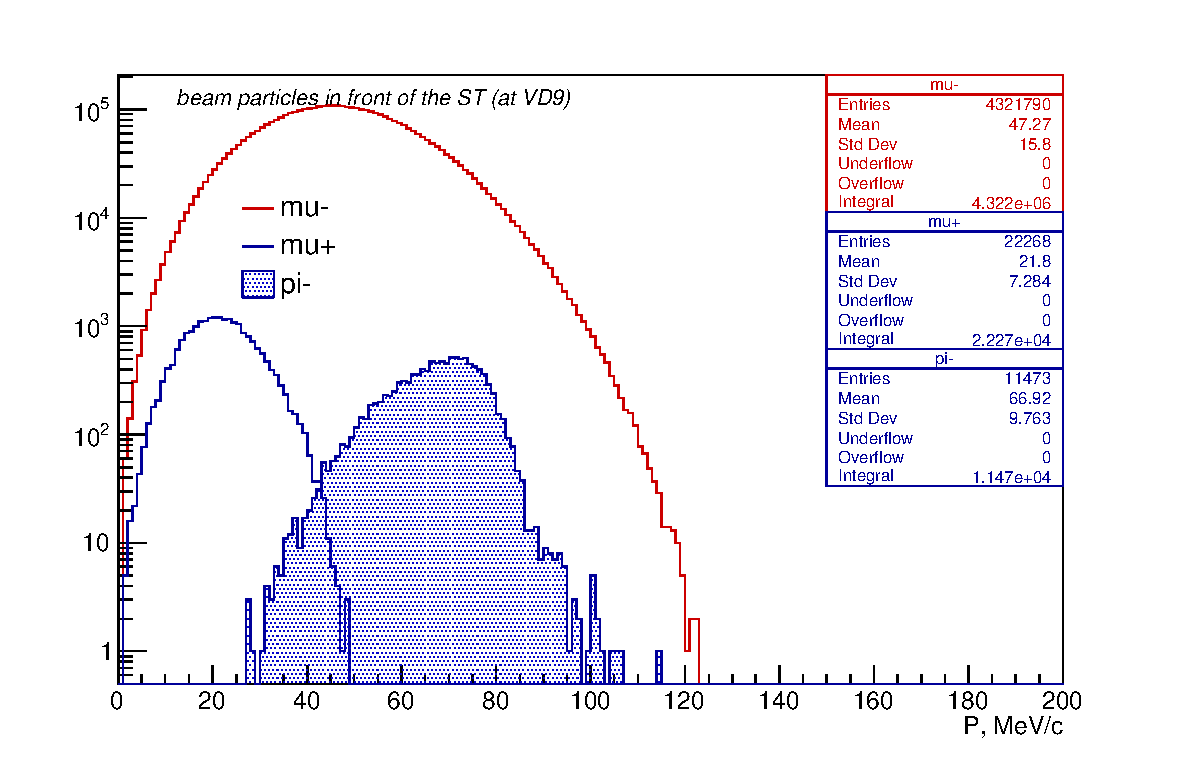
\includegraphics[width=0.6\textwidth]{figures/pdf/figure_03700_bmum0s37b0_vdet_xx09_mom}
      % }
    };
    \node[anchor=south west,inner sep=0] at (10,0.) {
      % \node[shift={(0 cm,0.cm)},inner sep=0,rotate={90}] at (0,0) {}
      % \makebox[\textwidth][c] {
      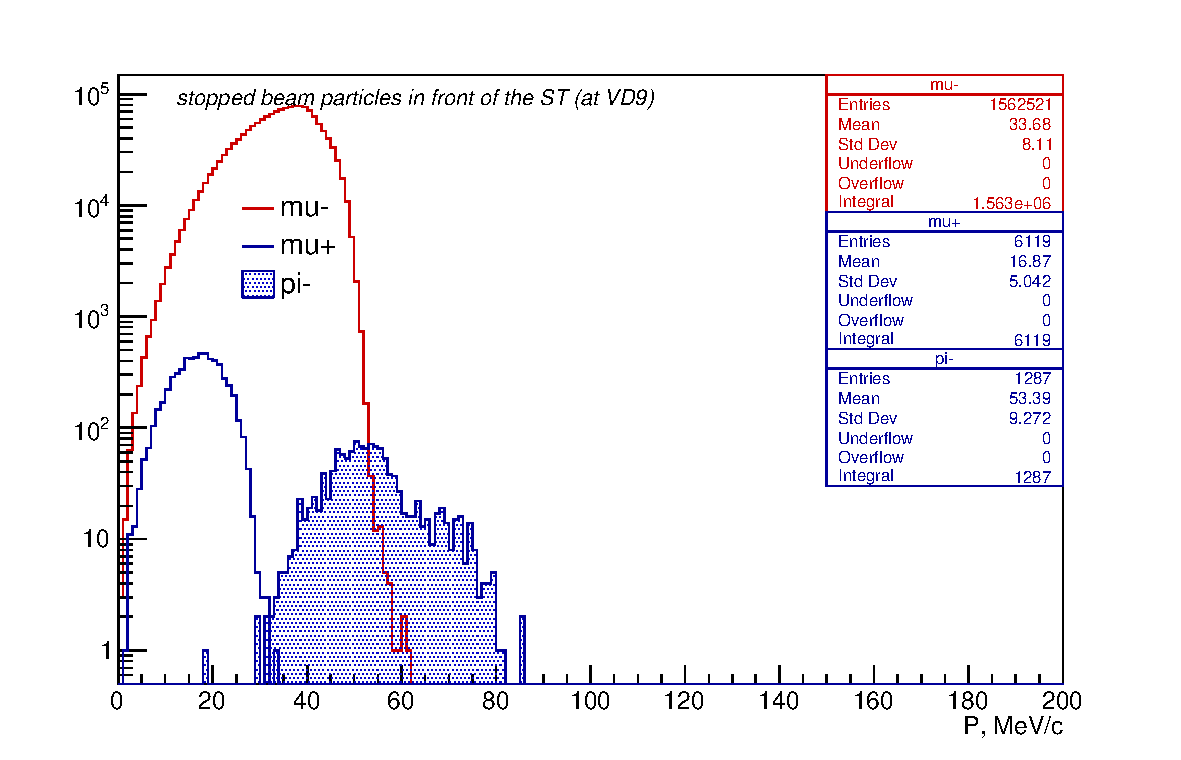
\includegraphics[width=0.6\textwidth]{figures/pdf/figure_03100_bmum0s31b0_vdet_xx09_mom}
      % }
    };
  \end{tikzpicture}
  \caption{
    \label{fig:03700_bmum0s37b0_vdet_xx09_mom}
    Left: momentum distributions of particles reaching VD9;
    Right: momentum distributions at VD9 of particles stopped in the stopping target
  }
\end{figure}

\begin{figure}[H]
  \hspace{-0.5in}
  \begin{tikzpicture}
    \node[anchor=south west,inner sep=0] at (0,0.) {
      % \node[shift={(0 cm,0.cm)},inner sep=0,rotate={90}] at (0,0) {}
      % \makebox[\textwidth][c] {
      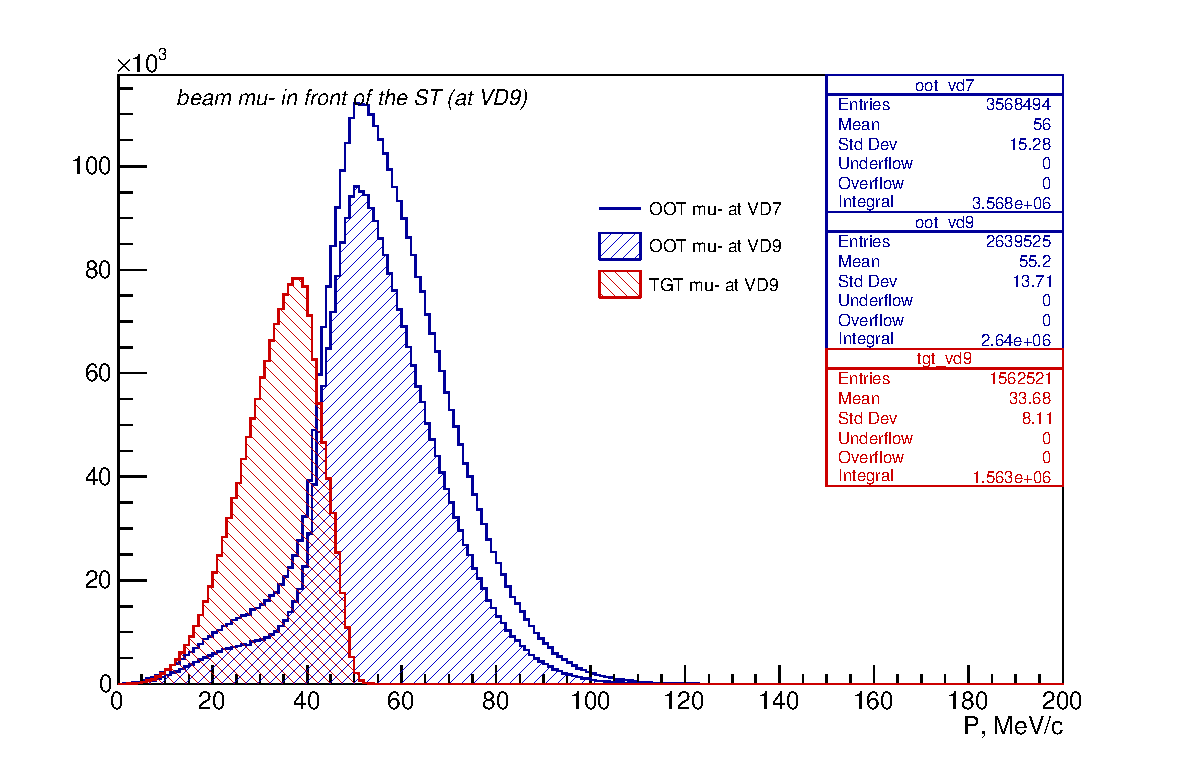
\includegraphics[width=0.60\textwidth]{figures/pdf/figure_03101_bmum0s31b0_vdet_x309_mom}
      % }
    };
    \node[anchor=south west,inner sep=0] at (10,0.) {
      % \node[shift={(0 cm,0.cm)},inner sep=0,rotate={90}] at (0,0) {}
      % \makebox[\textwidth][c] {
      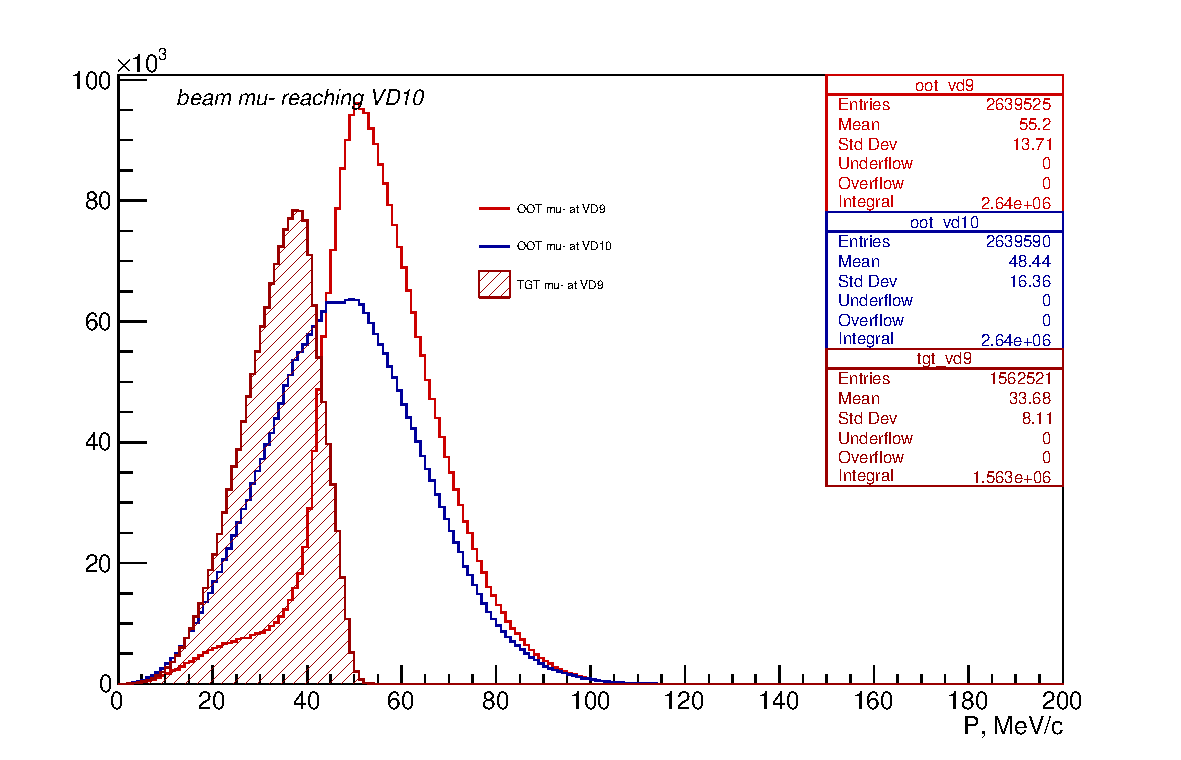
\includegraphics[width=0.60\textwidth]{figures/pdf/figure_03200_bmum0s32b0_vdet_0310_mom}
      % }
    };
  \end{tikzpicture}
  \caption{
    \label{fig:03101_bmum0s31b0_vdet_x309_mom}
    a... 
  }
\end{figure}

%%%%%%%%%%%%%%%%%%%%%%%%%%%%%%%%%%%%%%%%%%%%%%%%%%%%%%%%%%%%%%%%%%%%%%%%%%%%%%
\section {Muon Beamline Alignment}

One of the possible techniques could utilize the fact that the default position of the TS3 collimator does not reduce the \muplus \
transport efficiency down to zero.
%
As shown in Figure \ref{fig:03101_bmum0s31b0_vdet_x309_mom}, with the TS3 collimator 
in the default position, there still is a small fraction of $\mu^+$'s reaching
the stopping target and stopping there. The ratio of \muplus/\muminus stopping rates
is about 0.4\%.  
The ration can be measured by reconstructing electrons and positrons
from Michel decays in a reduced magnetic field.
%
The \muplus\ ``beam spot'' is offset vertically, its lower cut-off is determined by the opening
of the TS3 collimator.

\begin{figure}[H]
  \hspace{-0.5in}
  \begin{tikzpicture}
    \node[anchor=south west,inner sep=0] at (0,0.) {
      % \node[shift={(0 cm,0.cm)},inner sep=0,rotate={90}] at (0,0) {}
      % \makebox[\textwidth][c] {
      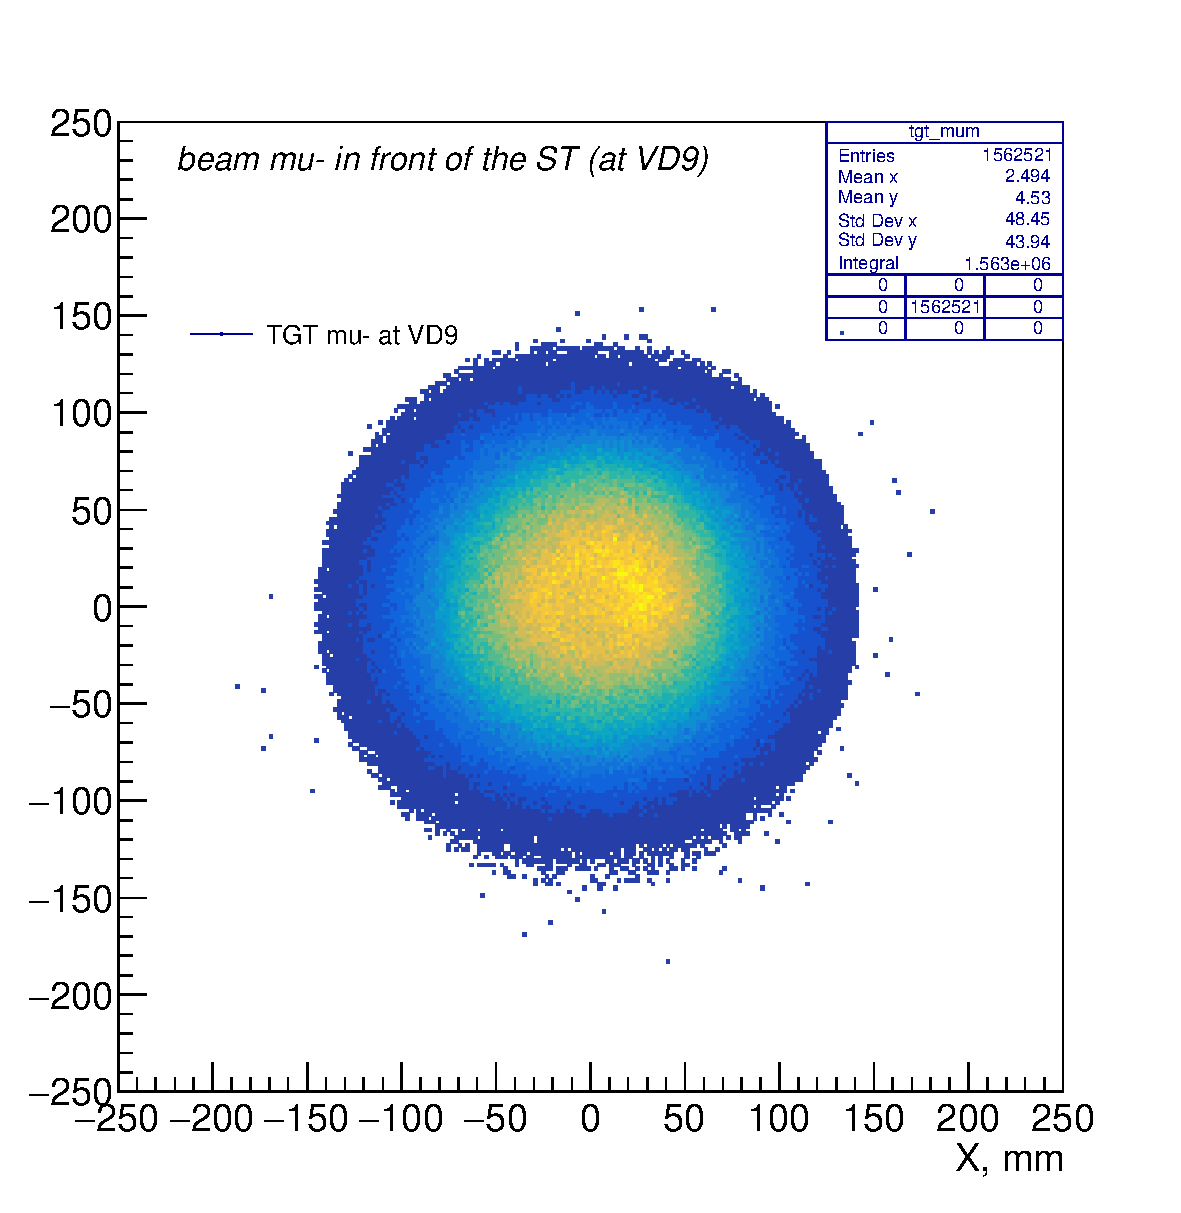
\includegraphics[width=0.5\textwidth]{figures/pdf/figure_03103_bmum0s31b0_vdet_309_y_vs_x}
      % }
    };
    \node[anchor=south west,inner sep=0] at (10,0.) {
      % \node[shift={(0 cm,0.cm)},inner sep=0,rotate={90}] at (0,0) {}
      % \makebox[\textwidth][c] {
      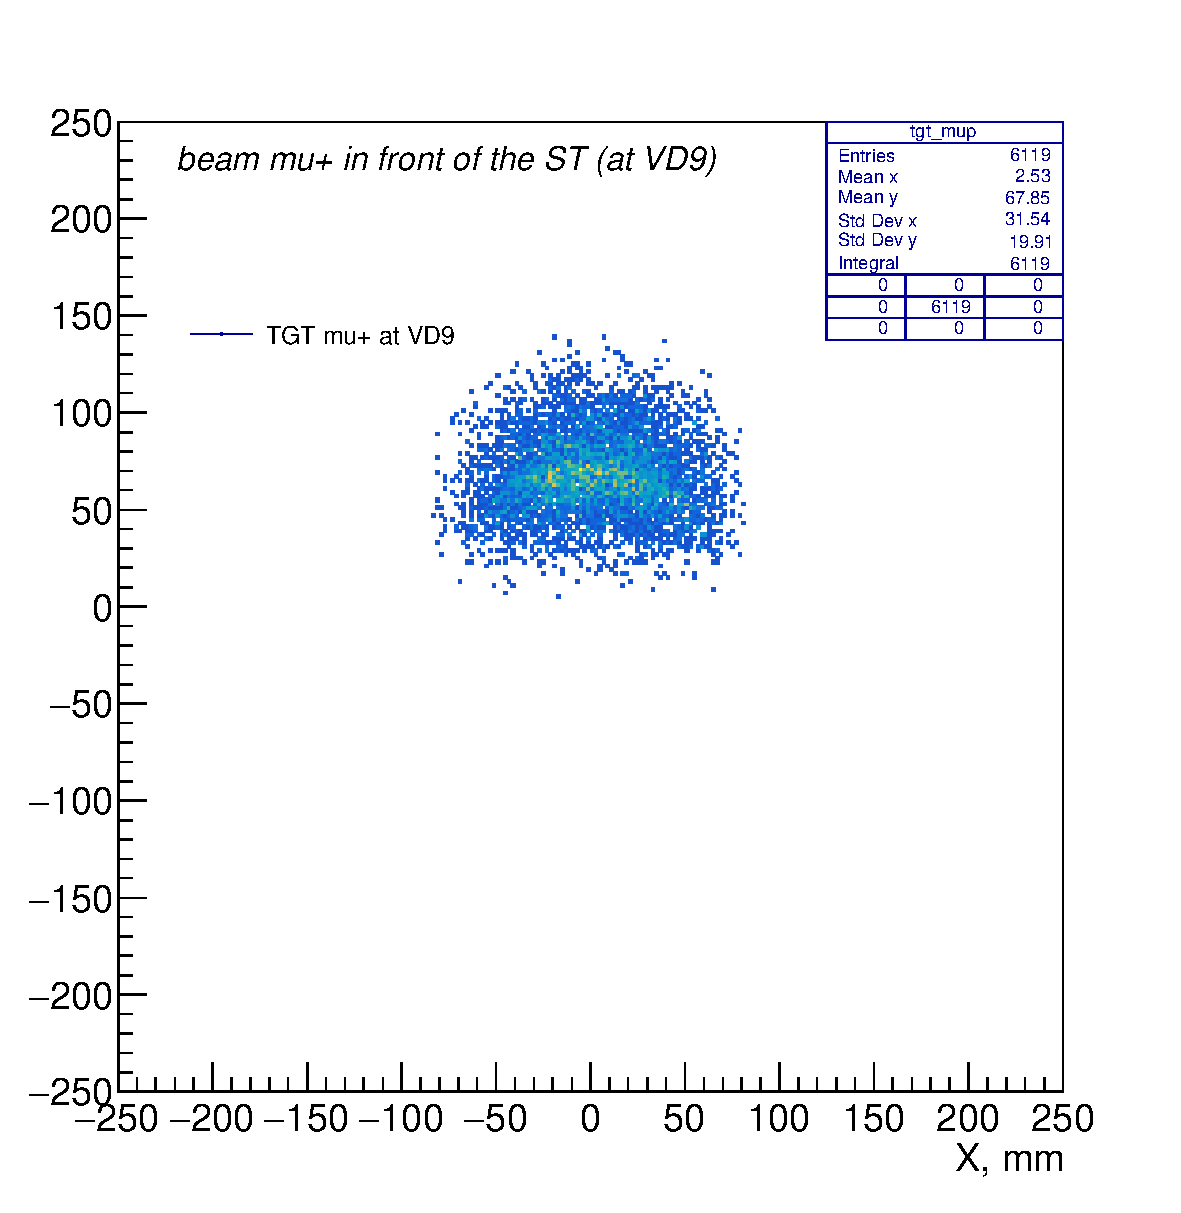
\includegraphics[width=0.5\textwidth]{figures/pdf/figure_03104_bmum0s31b0_vdet_409_y_vs_x}
      % }
    };
  \end{tikzpicture}
  \caption{
    \label{fig:03103_bmum0s31b0_vdet_309_y_vs_x}
    a ... 
  }
\end{figure}

Figure \ref{fig:03103_bmum0s31b0_vdet_309_y_vs_x} shows Y:X distributions at VD9 of \muminus's
and \muplus's stopped in the stopping target.

The vertical offset of the \muplus\ ``beam spot'' translates into a vertical offset of the illuminated
area of the stopping target. The low Y cut-off is defined by the vertical positions of the production target
and the TS3 collimator, and vertical misalignment of the TS3 collimator should therefore affect the ratio
of \muplus\ and \muminus\ stopping rates. 
%
Particle trajectories in the tracker are approximately helical. If we define the azimuthal angle
of the reconstructed trajectory as 
$$
\phi_0  ~=~ \arctan \frac{Y_0}{X_0}
$$
, where $X_0$ and $Y_0$ are the $x$ and $y$ coordinates of the helix axis,
the $\phi_0$ distribution for the reconstructed positrons should be asymmetric, 
with a maximum at around 90 degrees and a minimum around 270 degrees. 

The ratio of \muplus\ and \muminus stopping rates and the asymmetries of the \muplus\ and 
\muminus\ $\phi_0$ distributions are sensitive to the relative vertical positions
of the production target, TS3 collimator, and the stopping target. Measurement of those
parameters should help understanding the vertical alignment of the beamline.

The measurement should be performed with the B-field in the DS reduced to about 50\%
to have the high momentum edge of the $\mu \ra e\nu\nu$ spectrum within the tracker acceptance.

The measurement could be performed as a part of the Mu2e calibration program in the beginning
of the data taking.

Repeating the measurement with the TS3 collimator rotated by 180 degrees would add robustness
to the beamline alignment procedure.

In-situ technique of understanding the vertical alignment of the Mu2e beamline might lower 
requirements to the accuracy of the PS magnetic field calibration.

Two-dimensional distributions for the stop coordinates are shown in figure
\begin{figure}[H]
  \hspace{-0.5in}
  \begin{tikzpicture}
    \node[anchor=south west,inner sep=0] at (0,0.) {
      % \node[shift={(0 cm,0.cm)},inner sep=0,rotate={90}] at (0,0) {}
      % \makebox[\textwidth][c] {
      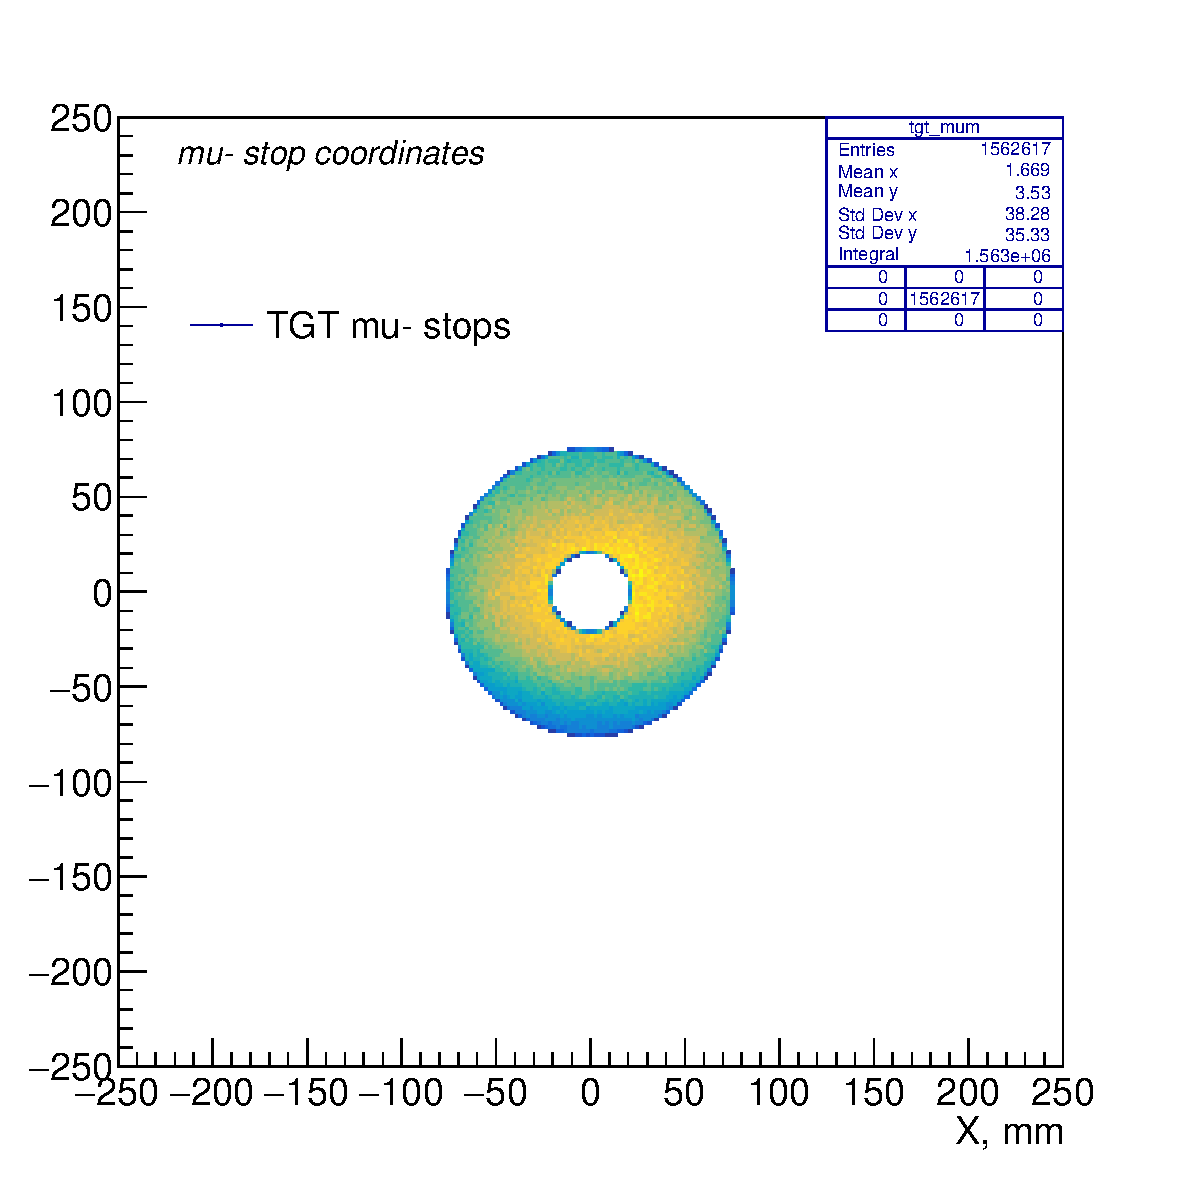
\includegraphics[width=0.5\textwidth]{figures/pdf/figure_03105_bmum0s31b0_simp_603_y_vs_x}
      % }
    };
    \node[anchor=south west,inner sep=0] at (10,0.) {
      % \node[shift={(0 cm,0.cm)},inner sep=0,rotate={90}] at (0,0) {}
      % \makebox[\textwidth][c] {
      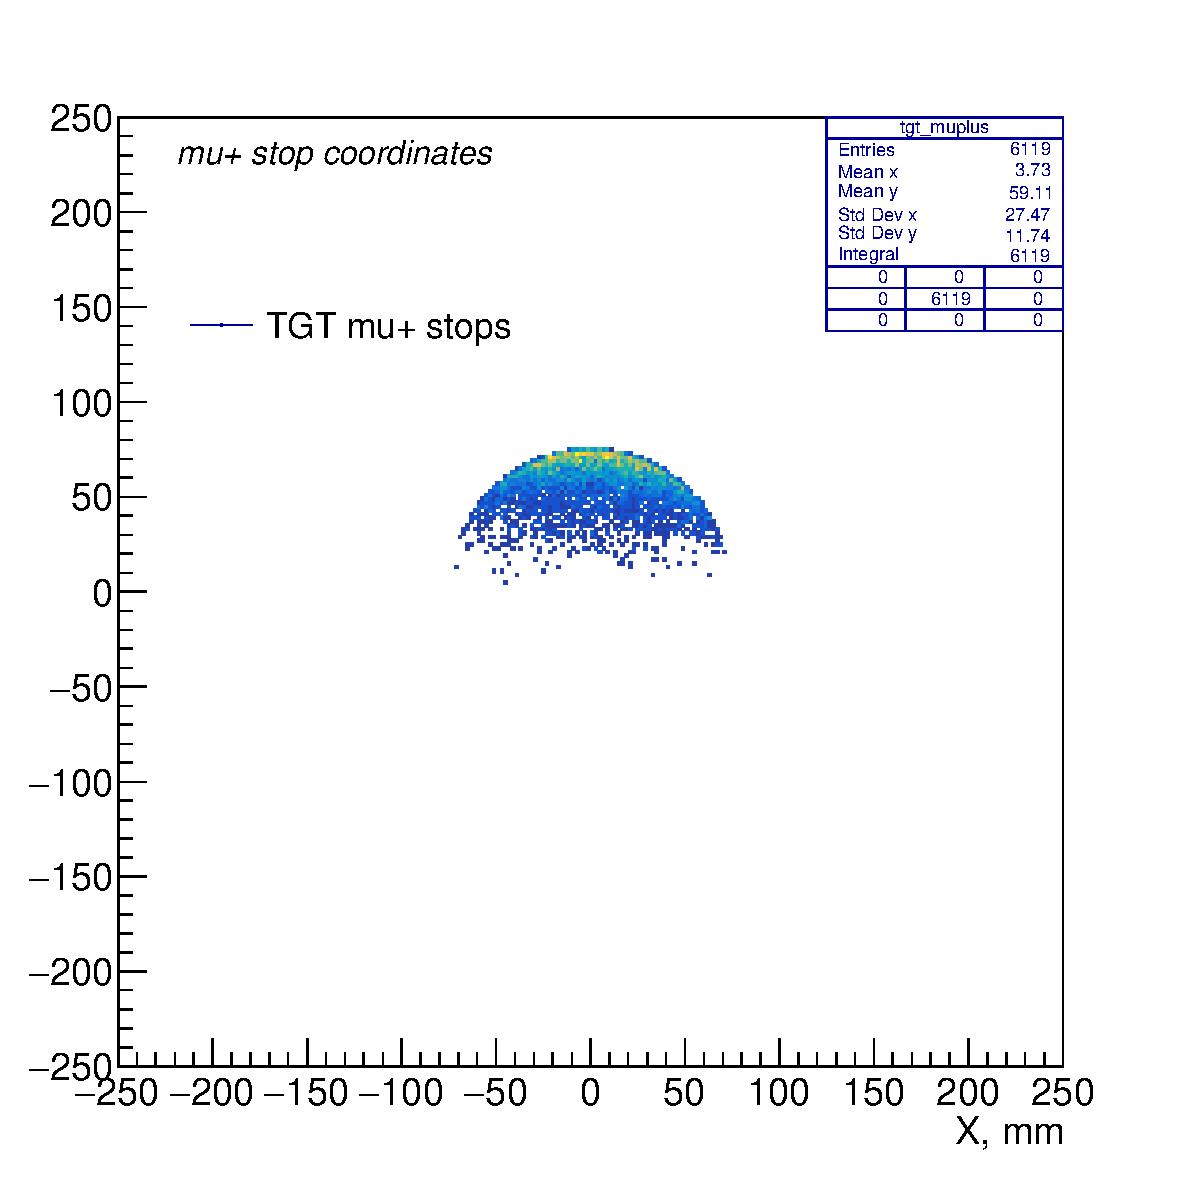
\includegraphics[width=0.5\textwidth]{figures/pdf/figure_03106_bmum0s31b0_simp_604_y_vs_x}
      % }
    };
  \end{tikzpicture}
  \caption{
    \label{fig:03103_bmum0s31b0_simp_603_y_vs_x}
    a ... 
  }
\end{figure}

%%%%%%%%%%%%%%%%%%%%%%%%%%%%%%%%%%%%%%%%%%%%%%%%%%%%%%%%%%%%%%%%%%%%%%%%%%%%%%
\appendix

\section{Appendix 1: Estimate of the data rate }

As each event contains several electron tracks of interest, triggering on positrons could be used.
With the beam intensity reduced by x1000, one expects 0.1 \muplus\ stops per microbunch, assuming
$\sim ~30\%$ acceptance, the probability for a microbunch data to have a reconstructed track is 0.03.
Factoring the Michel spectrum in should give another factor of $|sim$ 2, reducing the probability
down to 0.015. So running with the positron trigger only at this intensity, one could expect
a natural trigger rejection of the order of 100.

At this intensity, a typical number of \muminus\ stops per pulse is $\sim ~25$, and about
10 \muminus\ decays in orbit. 
%
About 1/3 of those decays produces tracks with 40 hits/track, corresponding to 120 hits per microbunch.
With 40 bytes (2 data packets) per hit, the total size of the tracker data is $\sim$ 5 kBytes/microbunch.  
Adding a factor of x2 to account for the total event size gives the estimate of the expected data rate 
$$
R ~=~ 10 ~({\rm kB/pulse}) \times 2 \times 10^3 ~=~ 2 \times 10^7 ~({\rm bytes/sec}) = 20 ~{\rm MB/sec}
$$

The data logging rate of 20 MB/sec could be sustained easily, so an hour of data taking at B=0.5 T
and a beam intensity reduced by a factor of 1000 should result in about 6M reconstructed $e^+$'s
from $\mu^+ \ra e^+ \nu \nu$ decays.
%

\scriptsize{
\begin{verbatim}
* ------------------------------------------------------------------------------
* estimate of the number of mu+ reconstructed per hour with the nominal collimator position      
#+begin_src maxima :results output
nppp                 : 1.6e7 ;                 /* number of protons per pulse              */
nmum_per_pot         : 1.6e-3;                 /* mu- stopping rate                        */
nmum_stops_per_pulse : nppp*nmum_per_pot;
nmup_stops_per_pulse : nppp*nmum_per_pot*4e-3;
                                               /*                                          */
                                               /* now : estimate the rate                  */
eff                  : 0.1;                    /* ballpark reco efficiency at 0.5 T        */
f_int                : 1e-3;                   /* beam intensity reduced by x1000          */
npulses_per_sec      : (1/1.695e-6)*0.4/1.4 ;  /* average pulse rate, account for beam-off */

nreco_per_hour       : nmup_stops_per_pulse*eff*f_int*npulses_per_sec*3600;

print("nmum_stops_per_pulse : ",nmum_stops_per_pulse);
print("nmup_stops_per_pulse : ",nmup_stops_per_pulse);
print("npulses_per_sec      : ",npulses_per_sec);
print("nreco_per_hour       : ",nreco_per_hour );
#+end_src

#+RESULTS:
: nmum_stops_per_pulse :  25600.0 
: nmup_stops_per_pulse :  102.4 
: npulses_per_sec      :  168563.0004214075 
: nreco_per_hour       :  6213906.447534768 
\end{verbatim}
}

%%%%%%%%%%%%%%%%%%%%%%%%%%%%%%%%%%%%%%%%%%%%%%%%%%%%%%%%%%%%%%%%%%%%%%%%%%%%%% 
\newpage
\section{Summary}

%%%%%%%%%%%%%%%%%%%%%%%%%%%%%%%%%%%%%%%%%%%%%%%%%%%%%%%%%%%%%%%%%%%%%%%%%%%%%%
%
%%%%%%%%%%%%%%%%%%%%%%%%%%%%%%%%%%%%%%%%%%%%%%%%%%%%%%%%%%%%%%%%%%%%%%%%%%%%%%
\newpage
\bibliographystyle{unsrtnat}
\bibliography{clfv,dio,mu2e_internal_notes}

\end{document}

%%%%%%%%%%%%%%%%%%%%%%%%%%%%%%%%%%%%%%%%%%%%%%%%%%%%%%%%%%%%%%%%%%%%%%%%%%%%%%
% small font sizes: \small \footnotesize \scriptsize \tiny
% ------------------------------------------------------------------------------
% templates
% ------------------------------------------------------------------------------
% Table ~\ref{table:summary} gives summary the numbers used in this study.
%
% \hspace{-0.1in}
% \begin{table}[htbp]
%   \label{table:summary}
%   \begin{center}
%     {\renewcommand{\arraystretch}{1.0}   % change 1.0 to 1.1 to increase the spacing between the table lines
%       \begin{tabular}{|c|c|c|c|}
%         \hline
%                             & default TS geometry & misaligned TS geometry   &  Ratio(default/misaligned)    \\
%         \hline
%         $N_{POT}$            &  $4.96 \cdot 10^6$  &    $5.00 \cdot 10^6$      &   0.992   \\
%         $N_{\mu}^{TS3u}$      &  65648              &     61354                 &   1.070   \\
%         $N_{\mu}^{TS5}$       &  28517              &     27351                 &   1.043   \\
%         $N_{\mu}^{ST}$        &  8868               &      8396                 &   1.056   \\
%         $N_{\mu}^{ST}/N_{POT}$ &  $1.79 \pm 0.02$    &    $1.68 \pm 0.02$        &   $1.065 \pm 0.03$        \\
%         \hline
%       \end{tabular}
%     }
%   \end{center}
%   \caption{
%     Muons rates at different points of the Mu2e beamline and stopping muon rates for nominal and
%     misaligned TS geometries
%   }
%   % \vspace{0.5in}
% \end{table}
